\documentclass[a4paper,12pt]{article}

\usepackage[T2A]{fontenc}
\usepackage[utf8]{inputenc}
\usepackage[russian]{babel}

\usepackage[margin=2cm]{geometry}
\usepackage{amsmath, amssymb}

\usepackage{graphicx}
\graphicspath{{assets}}

\usepackage{array}
\usepackage{float}
\usepackage{longtable}
\usepackage{multirow}
\usepackage{setspace}

\usepackage{hyperref}
\hypersetup{%
    colorlinks=true,
    linkcolor=blue,
    filecolor=magenta,
    urlcolor=magenta,
}

\setlength{\parindent}{0pt}

\newcommand\Section[1]{%
\refstepcounter{section}%
\section*{%
\raggedright
\arabic{section}. #1
}%
\addcontentsline{toc}{section}{\arabic{section}. #1}%
}

\newcommand\Subsection[1]{%
\refstepcounter{subsection}%
\subsection*{%
\raggedright%
\arabic{section}. \arabic{subsection}. #1
}%
\addcontentsline{toc}{subsection}{\arabic{subsection}. #1}%
}

\newcommand\Figure[4]{%
\refstepcounter{figure}%
\begin{figure}[H]
\begin{center}
\fbox{
\includegraphics[width=#2]{#1}
}
\end{center}
\begin{center}
Рис.~\arabic{figure}. #3.
\end{center}
\label{fig:#4}
\end{figure}
}

\begin{document}

% ---------- HEADER ----------

\begin{minipage}{0.55\textwidth}
    \begin{center}
        \textbf{Университет ИТМО}\\
        Физико-технический факультет\\
        Физический факультет
    \end{center}
\end{minipage}
\hfill
\begin{minipage}{0.35\textwidth}
    \begin{flushright}
        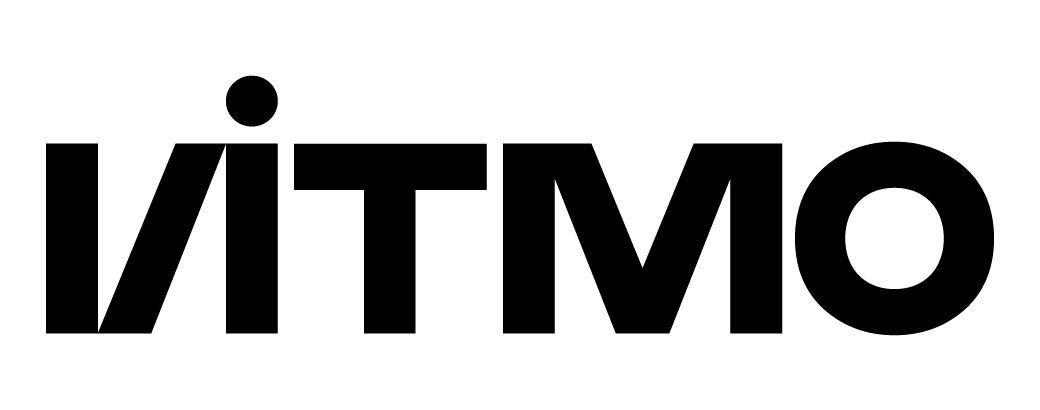
\includegraphics[width=3.2cm]{assets/itmo_logo.png}
    \end{flushright}
\end{minipage}

\vspace{1.2cm}

% ---------- INFORMATION ----------

\begin{tabular}{@{}p{7cm}p{6cm}@{}}

Группа\hspace{0.3cm}%
\makebox[4cm]{%
    \rlap{\raisebox{0.3ex}{\hspace{1.0cm}ПИИКТ 2.2}}%
    \hrulefill
}
&
К работе допущен \hrulefill
\\[0.8cm]

Студент\hspace{0.3cm}%
\makebox[4cm]{%
    \rlap{\raisebox{0.3ex}{\hspace{0.5cm}Бых Д. М.}}%
    \hrulefill
}
&
Работа выполнена \hrulefill
\\[0.8cm]

Преподаватель\hspace{0.2cm}%
\makebox[3cm]{%
    \rlap{\raisebox{0.3ex}{\hspace{0.5cm}Рудель А. Е.}}%
    \hrulefill
}
&
Отчет принят \hrulefill

\end{tabular}

\vspace{1.2cm}

% ---------- TITLE ----------

\begin{center}

{\Large\bfseries
Рабочий протокол и отчет по\\
лабораторной работе №1.02
}

\vspace{1cm}

{\large
\textit{Изучение скольжения тележки по наклонной плоскости}
}

\end{center}

\vspace{2cm}

\Section{Цель работы}
\begin{enumerate}
    \item Экспериментальная проверка равноускоренности движения тела по наклонной плоскости.
    \item Определение величины ускорения свободного падения.
\end{enumerate}

\Section{Задачи, решаемые при выполнении работы}
\begin{enumerate}
    \item Измерить зависимость времени движения от пройденного расстояния при движении тела по наклонной плоскости с фиксированным углом наклона.
    \item Измерить зависимость времени прохождения телом фиксированного расстояния от угла наклона плоскости к горизонту.
    \item Исследовать зависимость времени движения от пройденного расстояния при движении тела по наклонной плоскости при фиксированном угле наклона плоскости.
    \item Исследовать зависимость времени прохождения телом фиксированного расстояния от угла наклона рельса к горизонту.
    \item Исследовать зависимость ускорения тела от угла наклона рельса к горизонту.
\end{enumerate}

\Section{Объект исследования}
Тележка, скользящая по наклонной плоскости на воздушной подушке.

\Section{Метод экспериментального исследования}
Эксперимент, измерение.

\Section{Рабочие формулы и исходные данные}

Второй закон Ньютона для тележки:
\[
m\vec{a} = m\vec{g} + \vec{N} + \vec{F}_{\text{тр}},
\]
проекции на оси:
\[
\begin{cases}
0y: & 0 = N - mg\cos\alpha,\\
0x: & ma = mg\sin\alpha - F_{\text{тр}}.
\end{cases}
\]
Отсюда модуль ускорения:
\[
a = g\sin\alpha - \frac{F_{\text{тр}}}{m}.
\]

Кинематические соотношения:
\[
x(t) = x_0 + v_{0x}t + \frac{a_x t^2}{2},
\]
\[
x_2 - x_1 = \frac{a}{2}\left(t_2^2 - t_1^2\right).
\]
Обозначим
\[
Y = x_2 - x_1,\qquad Z = \frac{t_2^2 - t_1^2}{2}.
\]
Тогда
\[
Y = a Z,
\]
где \(a\) — ускорение тележки.

Для задания 2 синус угла наклона:
\[
\sin\alpha = \left|\frac{(h_0 - h) - (h_0' - h')}{X' - X}\right|.
\]
Среднее ускорение:
\[
\langle a\rangle = \frac{2(x_2 - x_1)}{\langle t_2\rangle^2 - \langle t_1\rangle^2}.
\]
Аппроксимация:
\[
a = A + B\sin\alpha,\qquad B = g.
\]
Коэффициенты \(A\) и \(B\) находятся методом наименьших квадратов:
\[
B = \frac{\sum a_i\sin\alpha_i - \frac{1}{n}\sum a_i\sum\sin\alpha_i}
{\sum\sin^2\alpha_i - \frac{1}{n}\left(\sum\sin\alpha_i\right)^2},
\]
\[
A = \frac{1}{n}\left(\sum a_i - B\sum\sin\alpha_i\right).
\]
СКО для \(g\):
\[
S_g = \sqrt{\frac{\sum d_i^2}{D(n-2)}},\qquad
d_i = a_i - (A + B\sin\alpha_i),\qquad
D = \sum\sin^2\alpha_i - \frac{1}{n}\left(\sum\sin\alpha_i\right)^2.
\]
Абсолютная погрешность:
\[
\Delta_g = 2S_g,\qquad \delta_g = \frac{\Delta_g}{g}\cdot100\%.
\]

\vspace{0.3cm}
\noindent\textbf{Исходные данные:}\\
\(\alpha = 0{,}95\) — доверительная вероятность;\\
\(n = 5\) — число измерений в каждой серии;\\
\(g_{\text{табл}} = 9{,}82\ \text{м/с}^2\) — табличное значение ускорения свободного падения для Санкт-Петербурга;\\
\(x_1 = 0{,}15\) м, \(x_2 = 1{,}10\) м (Задание 2);\\
\(h_0 = 174\) мм, \(h_0' = 174\) мм, \(X = 220\) мм, \(X' = 1000\) мм.

\Section{Измерительные приборы}
\begin{table}[h!]
    \centering
    \renewcommand{\arraystretch}{1.5}
    \begin{tabular}{|c|p{4.2cm}|p{2.6cm}|p{2.2cm}|p{1.8cm}|p{2.2cm}|}
        \hline
        \textit{№ п/п} & \centering\textit{Наименование} \arraybackslash & \centering\textit{Предел измерений} \arraybackslash & \centering\textit{Цена деления} \arraybackslash & \centering\textit{Класс точности} \arraybackslash & \centering\textit{Погрешность} \arraybackslash \tabularnewline
        \hline
        1 & Линейка на рельсе & 1{,}3 м & 1 см & -- & 5{,}0 мм \tabularnewline
        \hline
        2 & Линейка на угольнике & 250 мм & 1 мм & -- & 0{,}5 мм \tabularnewline
        \hline
        3 & Прибор ПКЦ-3 (режим секундомера) & 100 с & 0{,}1 с & -- & 0{,}1 с \tabularnewline
        \hline
    \end{tabular}
\end{table}

\Section{Схема установки}
\begin{figure}[H]
    \centering
    \fbox{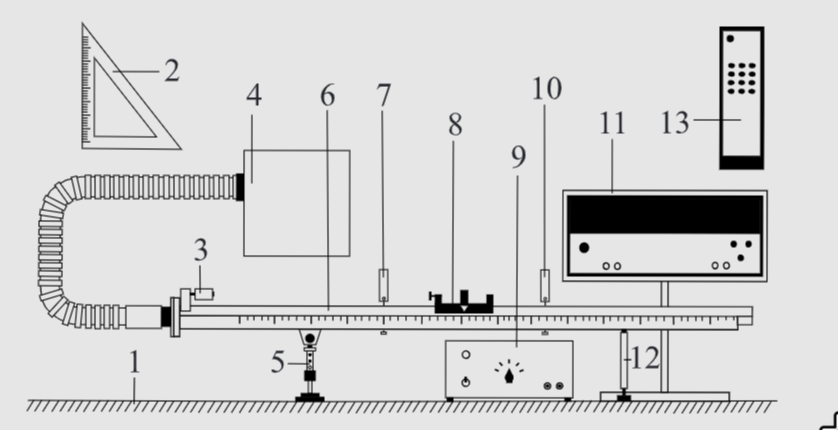
\includegraphics[width=0.8\textwidth]{assets/scheme.png}}
    \caption{Схема экспериментального стенда}
    \label{fig:scheme}
\end{figure}

\Section{Результаты прямых измерений и их обработки}

\Subsection{Задание 1. Исследование движения при фиксированном угле наклона}
\begin{table}[H]
    \centering
    \caption{Результаты измерений и расчёт \(Y\) и \(Z\)}
    \begin{tabular}{|c|c|c|c|c|c|c|}
        \hline
        № & \(x_1\), м & \(x_2\), м & \(t_1\), с & \(t_2\), с & \(Y=x_2-x_1\), м & \(Z=\frac{t_2^2-t_1^2}{2}\), с\(^2\) \\
        \hline
        1 & 0.15 & 0.40 & 1.3 & 2.5 & 0.25 & 2.280 \\
        \hline
        2 & 0.15 & 0.50 & 1.3 & 2.8 & 0.35 & 3.075 \\
        \hline
        3 & 0.15 & 0.70 & 1.3 & 3.4 & 0.55 & 4.935 \\
        \hline
        4 & 0.15 & 0.90 & 0.9 & 3.9 & 0.75 & 7.200 \\
        \hline
        5 & 0.15 & 1.10 & 1.4 & 4.5 & 0.95 & 9.145 \\
        \hline
    \end{tabular}
\end{table}

Пример расчёта для первой строки:
\[
Y = 0.40 - 0.15 = 0.25\ \text{м},\qquad
Z = \frac{2.5^2 - 1.3^2}{2} = \frac{6.25 - 1.69}{2} = 2.280\ \text{с}^2.
\]
Абсолютные погрешности (однократные измерения):
\[
\Delta_Y = \sqrt{2}\,\Delta_x \approx 0.0071\ \text{м},\qquad
\Delta_Z = \Delta_t\sqrt{t_1^2+t_2^2},\quad \Delta_t = 0.1\ \text{с}.
\]
Относительные погрешности:
\[
\delta_Y = \frac{\Delta_Y}{Y}\cdot100\%,\qquad
\delta_Z = \frac{\Delta_Z}{Z}\cdot100\%.
\]

\Subsection{Задание 2. Исследование зависимости ускорения от угла наклона}
\begin{table}[H]
    \centering
    \caption{Средние времена, синус угла и ускорение}
    \begin{tabular}{|c|c|c|c|c|c|c|c|}
        \hline
        № & \(h\), мм & \(h'\), мм & \(\sin\alpha\) & \(\langle t_1\rangle\), с & \(\langle t_2\rangle\), с & \(a\), м/с\(^2\) & \(\Delta_a\), м/с\(^2\) \\
        \hline
        1 & 183 & 174 & 0.01154 & 1.18 & 4.06 & 0.1259 & 0.0334 \\
        \hline
        2 & 193 & 175 & 0.02308 & 0.88 & 3.06 & 0.2212 & 0.0156 \\
        \hline
        3 & 203 & 177 & 0.03333 & 0.74 & 2.50 & 0.3332 & 0.0213 \\
        \hline
        4 & 213 & 178 & 0.04487 & 0.62 & 2.18 & 0.4350 & 0.0393 \\
        \hline
        5 & 223 & 179 & 0.05641 & 0.60 & 2.00 & 0.5220 & 0.0401 \\
        \hline
    \end{tabular}
\end{table}

Пример расчёта для первой серии:
\[
\sin\alpha = \frac{|183-174|}{1000-220} = \frac{9}{780} = 0.01154,
\]
\[
\langle t_1\rangle = \frac{1.3+1.0+1.2+1.2+1.2}{5} = 1.18\ \text{с},\qquad
\langle t_2\rangle = \frac{3.4+4.0+4.3+4.3+4.3}{5} = 4.06\ \text{с},
\]
\[
a = \frac{2\cdot(1.10-0.15)}{4.06^2 - 1.18^2} = \frac{1.9}{15.0912} = 0.1259\ \text{м/с}^2.
\]
Погрешность \(\Delta_a\) вычисляется по формуле (22) методички:
\[
\Delta a = \langle a\rangle \cdot \sqrt{\frac{2\Delta_x^2}{(x_2-x_1)^2} + 4\,\frac{(\langle t_1\rangle\Delta_{t1})^2 + (\langle t_2\rangle\Delta_{t2})^2}{(\langle t_2\rangle^2 - \langle t_1\rangle^2)^2}},
\]
где \(\Delta_{t} = \sqrt{\Delta_{(t)}^2 + \left(\tfrac{2}{3}\Delta_{\text{и}}\right)^2}\), \(\Delta_{(t)} = t_{\alpha,n}S(t)\).

\Section{Расчет результатов косвенных измерений}

\Subsection{Задание 1}
МНК для зависимости \(Y = aZ\) (через начало координат):
\[
a = \frac{\sum Z_iY_i}{\sum Z_i^2} = \frac{18.44825}{174.479275} = 0.10573\ \text{м/с}^2.
\]
СКО:
\[
S_a = \sqrt{\frac{\sum(Y_i - aZ_i)^2}{(n-1)\sum Z_i^2}} = 0.001654\ \text{м/с}^2.
\]
Абсолютная и относительная погрешности:
\[
\Delta_a = 2S_a = 0.00331\ \text{м/с}^2,\qquad
\delta_a = \frac{\Delta_a}{a}\cdot100\% = 3.13\%.
\]

\Subsection{Задание 2}
По формулам МНК:
\[
B = g = 9.0065\ \text{м/с}^2,\qquad A = 0.02262\ \text{м/с}^2.
\]
СКО для \(g\):
\[
S_g = \sqrt{\frac{\sum d_i^2}{D(n-2)}} = 0.30036\ \text{м/с}^2.
\]
Абсолютная и относительная погрешности:
\[
\Delta_g = 2S_g = 0.6007\ \text{м/с}^2,\qquad
\delta_g = \frac{\Delta_g}{g}\cdot100\% = 6.67\%.
\]
Сравнение с табличным значением:
\[
|g - g_{\text{табл}}| = |9.0065 - 9.82| = 0.814\ \text{м/с}^2,\qquad
\varepsilon = \frac{0.814}{9.82}\cdot100\% = 8.29\%.
\]

\Section{Графики}
\begin{enumerate}
    \item График зависимости \(Y = f(Z)\) (см. рис.~\ref{fig:task1}).
    \item График зависимости \(a = f(\sin\alpha)\) (см. рис.~\ref{fig:task2}).
\end{enumerate}

\Section{Окончательные результаты}
\begin{enumerate}
    \item Ускорение тележки при фиксированном угле наклона:
    \[
    a = (0.1057 \pm 0.0033)\ \text{м/с}^2.
    \]
    \item Относительная погрешность ускорения тележки:
    \[
    \delta_a = \frac{\Delta_a}{a}\cdot100\% = 3.13\%.
    \]
    \item Ускорение свободного падения:
    \[
    g = (9.01 \pm 0.60)\ \text{м/с}^2.
    \]
    \item Относительная погрешность \(g\):
    \[
    \delta_g = \frac{\Delta_g}{g}\cdot100\% = 6.67\%.
    \]
    \item Абсолютное и относительное отклонения от табличного значения \(g_{\text{табл}} = 9.82\) м/с\(^2\):
    \[
    \Delta = 0.81\ \text{м/с}^2,\qquad \varepsilon = 8.29\%.
    \]
\end{enumerate}

\Section{Выводы и анализ результатов работы}
В ходе работы экспериментально подтверждена равноускоренность движения тележки по наклонной плоскости: зависимость \(Y(Z)\), представленная на рис.~\ref{fig:task1}, с хорошей точностью описывается линейной функцией, проходящей через начало координат (в пределах погрешности). Полученное ускорение тележки при фиксированном угле наклона составило \((0.1057 \pm 0.0033)\) м/с\(^2\).

При исследовании зависимости ускорения от угла наклона (рис.~\ref{fig:task2}) получено значение ускорения свободного падения \(g = (9.01 \pm 0.60)\) м/с\(^2\). Отличие от табличного значения для Санкт-Петербурга (9.82 м/с\(^2\)) составляет \(8.29\%\), что не превышает удвоенной относительной погрешности (\(2\delta_g = 13.3\%\)). Основными источниками погрешности являются: остаточное трение при движении тележки, погрешности измерения времени прибором ПКЦ-3 и координат линейкой, а также приближённость модели (сила трения считалась постоянной).

\Section{Дополнительные задания}

\Section{Выполнение дополнительных заданий}

\Section{Замечания преподавателя}
\vspace{2cm}

\newpage
\section*{Приложения}

\subsection*{Приложение 1. Результаты задания 1}
\begin{longtable}{|c|c|c|c|c|c|}
\hline
№ & \(Y\), м & \(\Delta_Y\), м & \(\delta_Y\), \% & \(Z\), с\(^2\) & \(\Delta_Z\), с\(^2\) \\
\hline
1 & 0.25 & 0.0071 & 2.83 & 2.280 & 0.282 \\
\hline
2 & 0.35 & 0.0071 & 2.02 & 3.075 & 0.309 \\
\hline
3 & 0.55 & 0.0071 & 1.29 & 4.935 & 0.364 \\
\hline
4 & 0.75 & 0.0071 & 0.94 & 7.200 & 0.400 \\
\hline
5 & 0.95 & 0.0071 & 0.74 & 9.145 & 0.471 \\
\hline
\end{longtable}

\subsection*{Приложение 2. Результаты задания 2}
\begin{longtable}{|c|c|c|c|c|c|}
\hline
№ & \(\sin\alpha\) & \(\langle t_1\rangle\), с & \(\Delta_{t1}\), с & \(\langle t_2\rangle\), с & \(\Delta_{t2}\), с \\
\hline
1 & 0.01154 & 1.18 & 0.152 & 4.06 & 0.491 \\
\hline
2 & 0.02308 & 0.88 & 0.087 & 3.06 & 0.095 \\
\hline
3 & 0.03333 & 0.74 & 0.095 & 2.50 & 0.067 \\
\hline
4 & 0.04487 & 0.62 & 0.087 & 2.18 & 0.087 \\
\hline
5 & 0.05641 & 0.60 & 0.067 & 2.00 & 0.067 \\
\hline
\end{longtable}

\subsection*{Приложение 3. Графики}
\begin{figure}[H]
    \centering
    \fbox{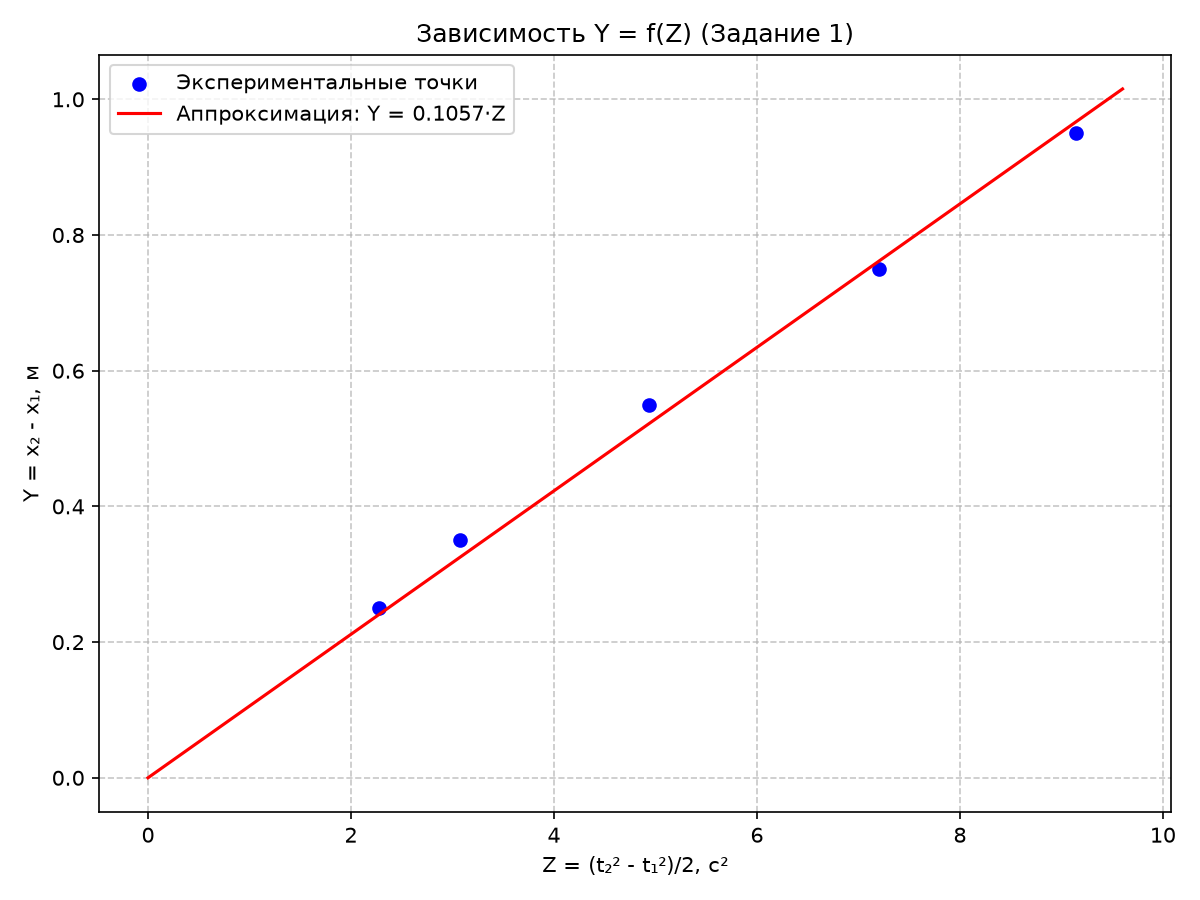
\includegraphics[width=0.8\textwidth]{assets/task1_graph.png}}
    \caption{Зависимость \(Y = f(Z)\)}
    \label{fig:task1}
\end{figure}

\begin{figure}[H]
    \centering
    \fbox{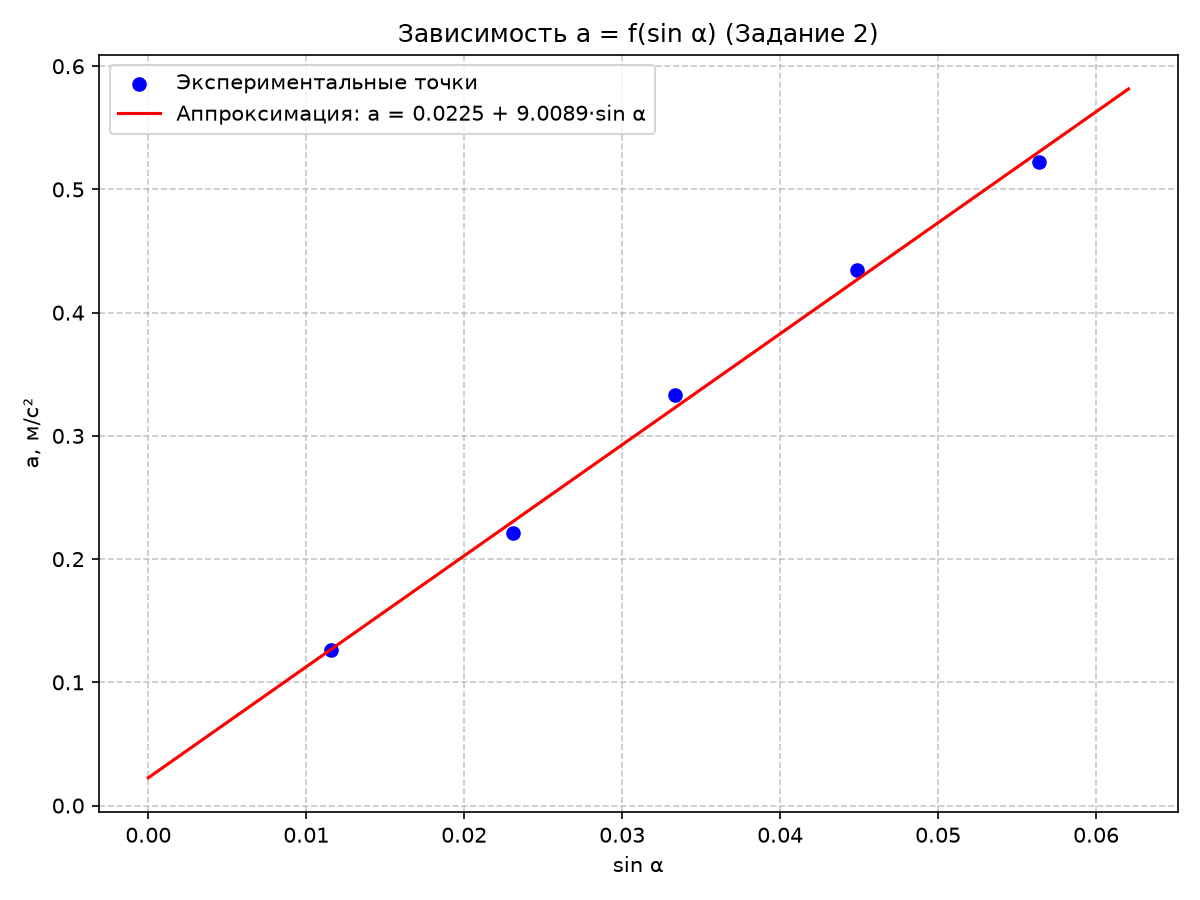
\includegraphics[width=0.8\textwidth]{assets/task2_graph.png}}
    \caption{Зависимость \(a = f(\sin\alpha)\)}
    \label{fig:task2}
\end{figure}

\end{document}